\documentclass[a4paper,addpoints]{exam}

\usepackage{amsfonts,amsmath,amsthm}
\usepackage[a4paper]{geometry}
\usepackage[table]{xcolor}
\usepackage{tikz}
\usetikzlibrary{positioning}

\header{CS/MATH 113}{WC15: Matching in Bipartite Graphs}{Spring 2024}
\footer{}{Page \thepage\ of \numpages}{}
\runningheadrule
\runningfootrule

\usepackage{draftwatermark}
\SetWatermarkText{Sample Solution}
\SetWatermarkScale{3}
\SetWatermarkLightness{.95}

\printanswers

\qformat{{\large\bf \thequestion. \thequestiontitle}\hfill(\totalpoints\ points)}
\boxedpoints

\title{Weekly Challenge 15: Matching in Bipartite Graphs}
\author{CS/MATH 113 Discrete Mathematics}
\date{Spring 2024}

\begin{document}
\maketitle

\begin{questions}
\titledquestion{$n$-doku}
  Let us define an $n$-doku as an $n\times n$ grid which contains all the numbers from $1$ to $n$ inclusive in the following manner.
  \begin{itemize}
  \item Each number appears exactly $n$ times in the grid.
  \item Each number appears exactly once in each row of the grid.
  \item Each number appears exactly once in each column of the grid.
  \end{itemize}
  For example here is a 4-doku.
  
  \begin{center}
    \begin{tabular}{|c|c|c|c|} \hline 
      4&  3&  1& 2\\ \hline
      3&  4&  2& 1\\ \hline 
      2&  1&  4& 3\\ \hline 
      1&  2&  3& 4\\ \hline 
    \end{tabular}
  \end{center}
  
  \begin{parts}
  \part[2] Below is a partially completed 5-doku.
    
    \begin{center}
      \begin{tabular}{|c|c|c|c|c|} \hline 
        1&  2&  5&  3& 4\\ \hline 
        3&  5&  2&  4& 1\\ \hline 
        5&  1&  4&  2& 3\\ \hline 
         &  &  &  & \\ \hline 
         &  &  &  & \\ \hline
      \end{tabular}
    \end{center}
    
    Copy and complete the 5-doku.
    \begin{solution}
      One possible solution is given below. Other solutions also exist.
      \begin{center}
        \begin{tabular}{|c|c|c|c|c|} \hline 
          1&  2&  5&  3& 4\\ \hline 
          3&  5&  2&  4& 1\\ \hline 
          5&  1&  4&  2& 3\\ \hline
          \rowcolor{lightgray}
          2&  4&  3&  1& 5\\ \hline 
          \rowcolor{lightgray}
          4&  3&  1&  5& 2\\ \hline
        \end{tabular}
      \end{center}
    \end{solution}
    
  \part[4] Show that filling in the next row of an $n$-doku is equivalent to finding a matching in some 2n-vertex bipartite graph.
    \begin{solution}
      Let the bipartite graph be $G$ with $C$ and $R$ as the bi-paritions. Each vertex in $C$ represents a column of the $n$-doku and contains all the numbers that appear in the column. As there are $n$ columns in the $n$-doku, there are $n$ vertices in $C$. There are $n$ vertices in $R$ corresponding to the numbers from $1$ to $n$. These represent the numbers to be filled in the first empty row.

      Filling the first empty row is a matter of deciding the next number in each column. This can be modeled as a matching from $C$ to $R$ under the constraint that a vertex, $c$, in $C$ does not connect with any vertex, $r$ in $R$ that represents any of the contained numbers in $c$.

      To illustrate, below is the graph and matching corresponding to the filling of the first empty row in the previous part.
      \begin{center}
        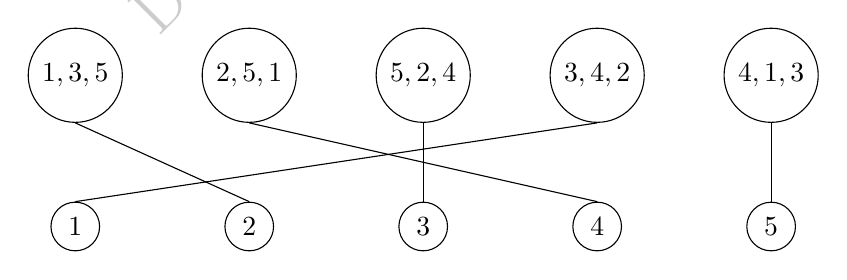
\begin{tikzpicture}
          \node[draw, circle] (c1) {$1,3,5$};
          \node[draw, circle, right = of c1] (c2) {$2,5,1$};
          \node[draw, circle, right = of c2] (c3) {$5,2,4$};
          \node[draw, circle, right = of c3] (c4) {$3,4,2$};
          \node[draw, circle, right = of c4] (c5) {$4,1,3$};
          \node[draw, circle, below = of c1] (n1) {$1$};
          \node[draw, circle, below = of c2] (n2) {$2$};
          \node[draw, circle, below = of c3] (n3) {$3$};
          \node[draw, circle, below = of c4] (n4) {$4$};
          \node[draw, circle, below = of c5] (n5) {$5$};

          \draw [-] (c1.south) -- (n2.north);
          \draw [-] (c2.south) -- (n4.north);
          \draw [-] (c3.south) -- (n3.north);
          \draw [-] (c4.south) -- (n1.north);
          \draw [-] (c5.south) -- (n5.north);
        \end{tikzpicture}
      \end{center}

      And below is the corresponding diagram for the next step, i.e., filling the last empty row in the previous part.
      \begin{center}
        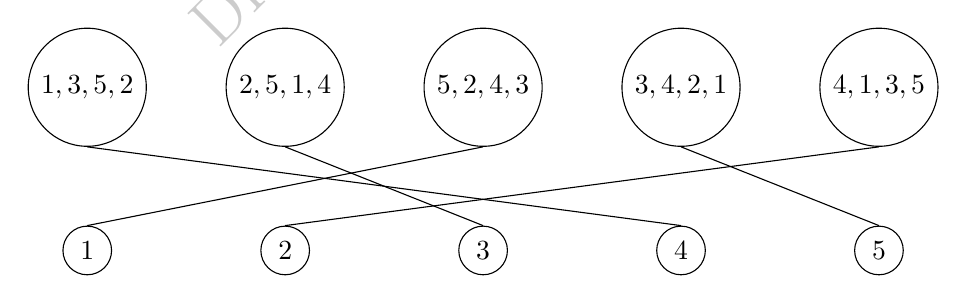
\begin{tikzpicture}
          \node[draw, circle] (c1) {$1,3,5,2$};
          \node[draw, circle, right = of c1] (c2) {$2,5,1,4$};
          \node[draw, circle, right = of c2] (c3) {$5,2,4,3$};
          \node[draw, circle, right = of c3] (c4) {$3,4,2,1$};
          \node[draw, circle, right = of c4] (c5) {$4,1,3,5$};
          \node[draw, circle, below = of c1] (n1) {$1$};
          \node[draw, circle, below = of c2] (n2) {$2$};
          \node[draw, circle, below = of c3] (n3) {$3$};
          \node[draw, circle, below = of c4] (n4) {$4$};
          \node[draw, circle, below = of c5] (n5) {$5$};

          \draw [-] (c1.south) -- (n4.north);
          \draw [-] (c2.south) -- (n3.north);
          \draw [-] (c3.south) -- (n1.north);
          \draw [-] (c4.south) -- (n5.north);
          \draw [-] (c5.south) -- (n2.north);
        \end{tikzpicture}
      \end{center}
    \end{solution}
    
  \part[4] Prove that a matching must exist in this bipartite graph and, consequently, that an incomplete $n$-doku can always be completed.
    \begin{solution}
      A matching always exists in a general $n\times n$ bipartite graph. However, as our matching depends on the content of the vertices, it is possible that some content makes a matching impossible. We will show that any such content cannot exist under the rules of the game.

      \begin{proof} A condition that makes a matching impossible cannot exist.

        \underline{Case 1}: A node $c\in C$ contains all the numbers, $1$ to $n$, so cannot match a $r\in R$.\\
        \textit{Proof by contradiction}.\\
        If this condition holds, then the column corresponding to $c$ is full. \\
        That is, the next row contains a number for this column.\\
        This is a contradiction, as the next row is supposed to be empty.\\
        Therefore, this condition cannot exist.
        
        \underline{Case 2}: Distinct nodes $c_1,c_2\in C$ must match the same $r\in R$.\\
        \textit{Proof by contradiction}.\\
        If this condition holds, then, $c_1$ and $c_2$ must each contain all the $n$ numbers except the number contained in $r$.\\
        \textit{wlog} let $c_1$ and $c_2$ contain the numbers from $1$ to $n-1$, so $r$ contains the number, $n$.\\
        $c_1$ and $c_2$ each contain $n-1$ numbers, so the first $n-1$ rows of the $n$-doku are full and only the last row remains to be filled.\\
        Among the first $n-1$ rows, the number, $n$, does not appear in 2 of the columns, namely $c_1$ or $c_2$.\\
        So, among the first $n-1$ rows, there are $n-2$ different columns in which the number $n$ may appear.\\
        This contradicts the rules of $n$-doku, according to which, in $n-1$ rows, any number must appear in $n-1$ different columns.\\
        Therefore, this condition cannot exist.
      \end{proof}
    \end{solution}
  \end{parts}
\end{questions}

\end{document}
%%% Local Variables:
%%% mode: latex
%%% TeX-master: t
%%% End: